\documentclass{instructions}

\usepackage{xspace}

\newcommand{\git}{\texttt{git}\xspace}
\newcommand\bs{\char`\\}

\graphicspath{{figs/}}

\title{Practical 2: Build a DC motor}
\date{\today}

\summary{
    Let's build a DC motor from scratch! You have \textbf{2 weeks} to: (1) build
    a first version, (2) iterate and optimise the design, (3) build a better
    version of your motor.
}

\objectives{
At the end of the practical, you should:

\begin{itemize}
    \item know the key parts of a DC motor
    \item have gained an experimental intuition of the physics behind DC motors
    \item have a working and reasonably efficient DC motor that we will re-use
        during the coming practicals
\end{itemize}
}

\challenges{

    \begin{itemize}
        \item A certain sense of meticulousness might be needed for an optimal
            result
        \item You'll get your hands dirty
        \item (and you'll need to use a soldering iron)
    \end{itemize}
}

\begin{document}

\maketitle


\note{
In your lab journal, \textbf{describe the basic design of each component},
\textbf{how it was constructed} and \textbf{how it was tested}. Add
\textbf{pictures} and link to \textbf{videos} as needed.

Describe as well \textbf{the overall system} and how it performs.

\vspace{1em}

And do not forget: \textbf{write your lab journal as a text file using the Markdown
syntax} and \textbf{push your journal and the pictures on GitHub}.

}

%%%%%%%%%%%%%%%%%%%%%%%%%%%%%%%%%%%%%%%%%%%%%%%%%%%%%%%%%%%%%%%%%%
%%%%%%%%%%%%%%%%%%%%%%%%%%%%%%%%%%%%%%%%%%%%%%%%%%%%%%%%%%%%%%%%%%
%%%%%%%%%%%%%%%%%%%%%%%%%%%%%%%%%%%%%%%%%%%%%%%%%%%%%%%%%%%%%%%%%%


\part{Build a brushed DC electrical motor}

In this assignment you will build a brushed DC motor from first
principles. Photos of a suggested design are provided in each section.

You need to build the motor working in pairs. You will be supplied with
a wooden base, a cork, and copper tape and about of 10m enamelled copper
wire. In addition you are provided with some paper clips, screws and
washer to hold everything together. You also will be supplied with 4
neodymium magnets.


\step{Build a commutator}

\begin{figure}
    \centering
    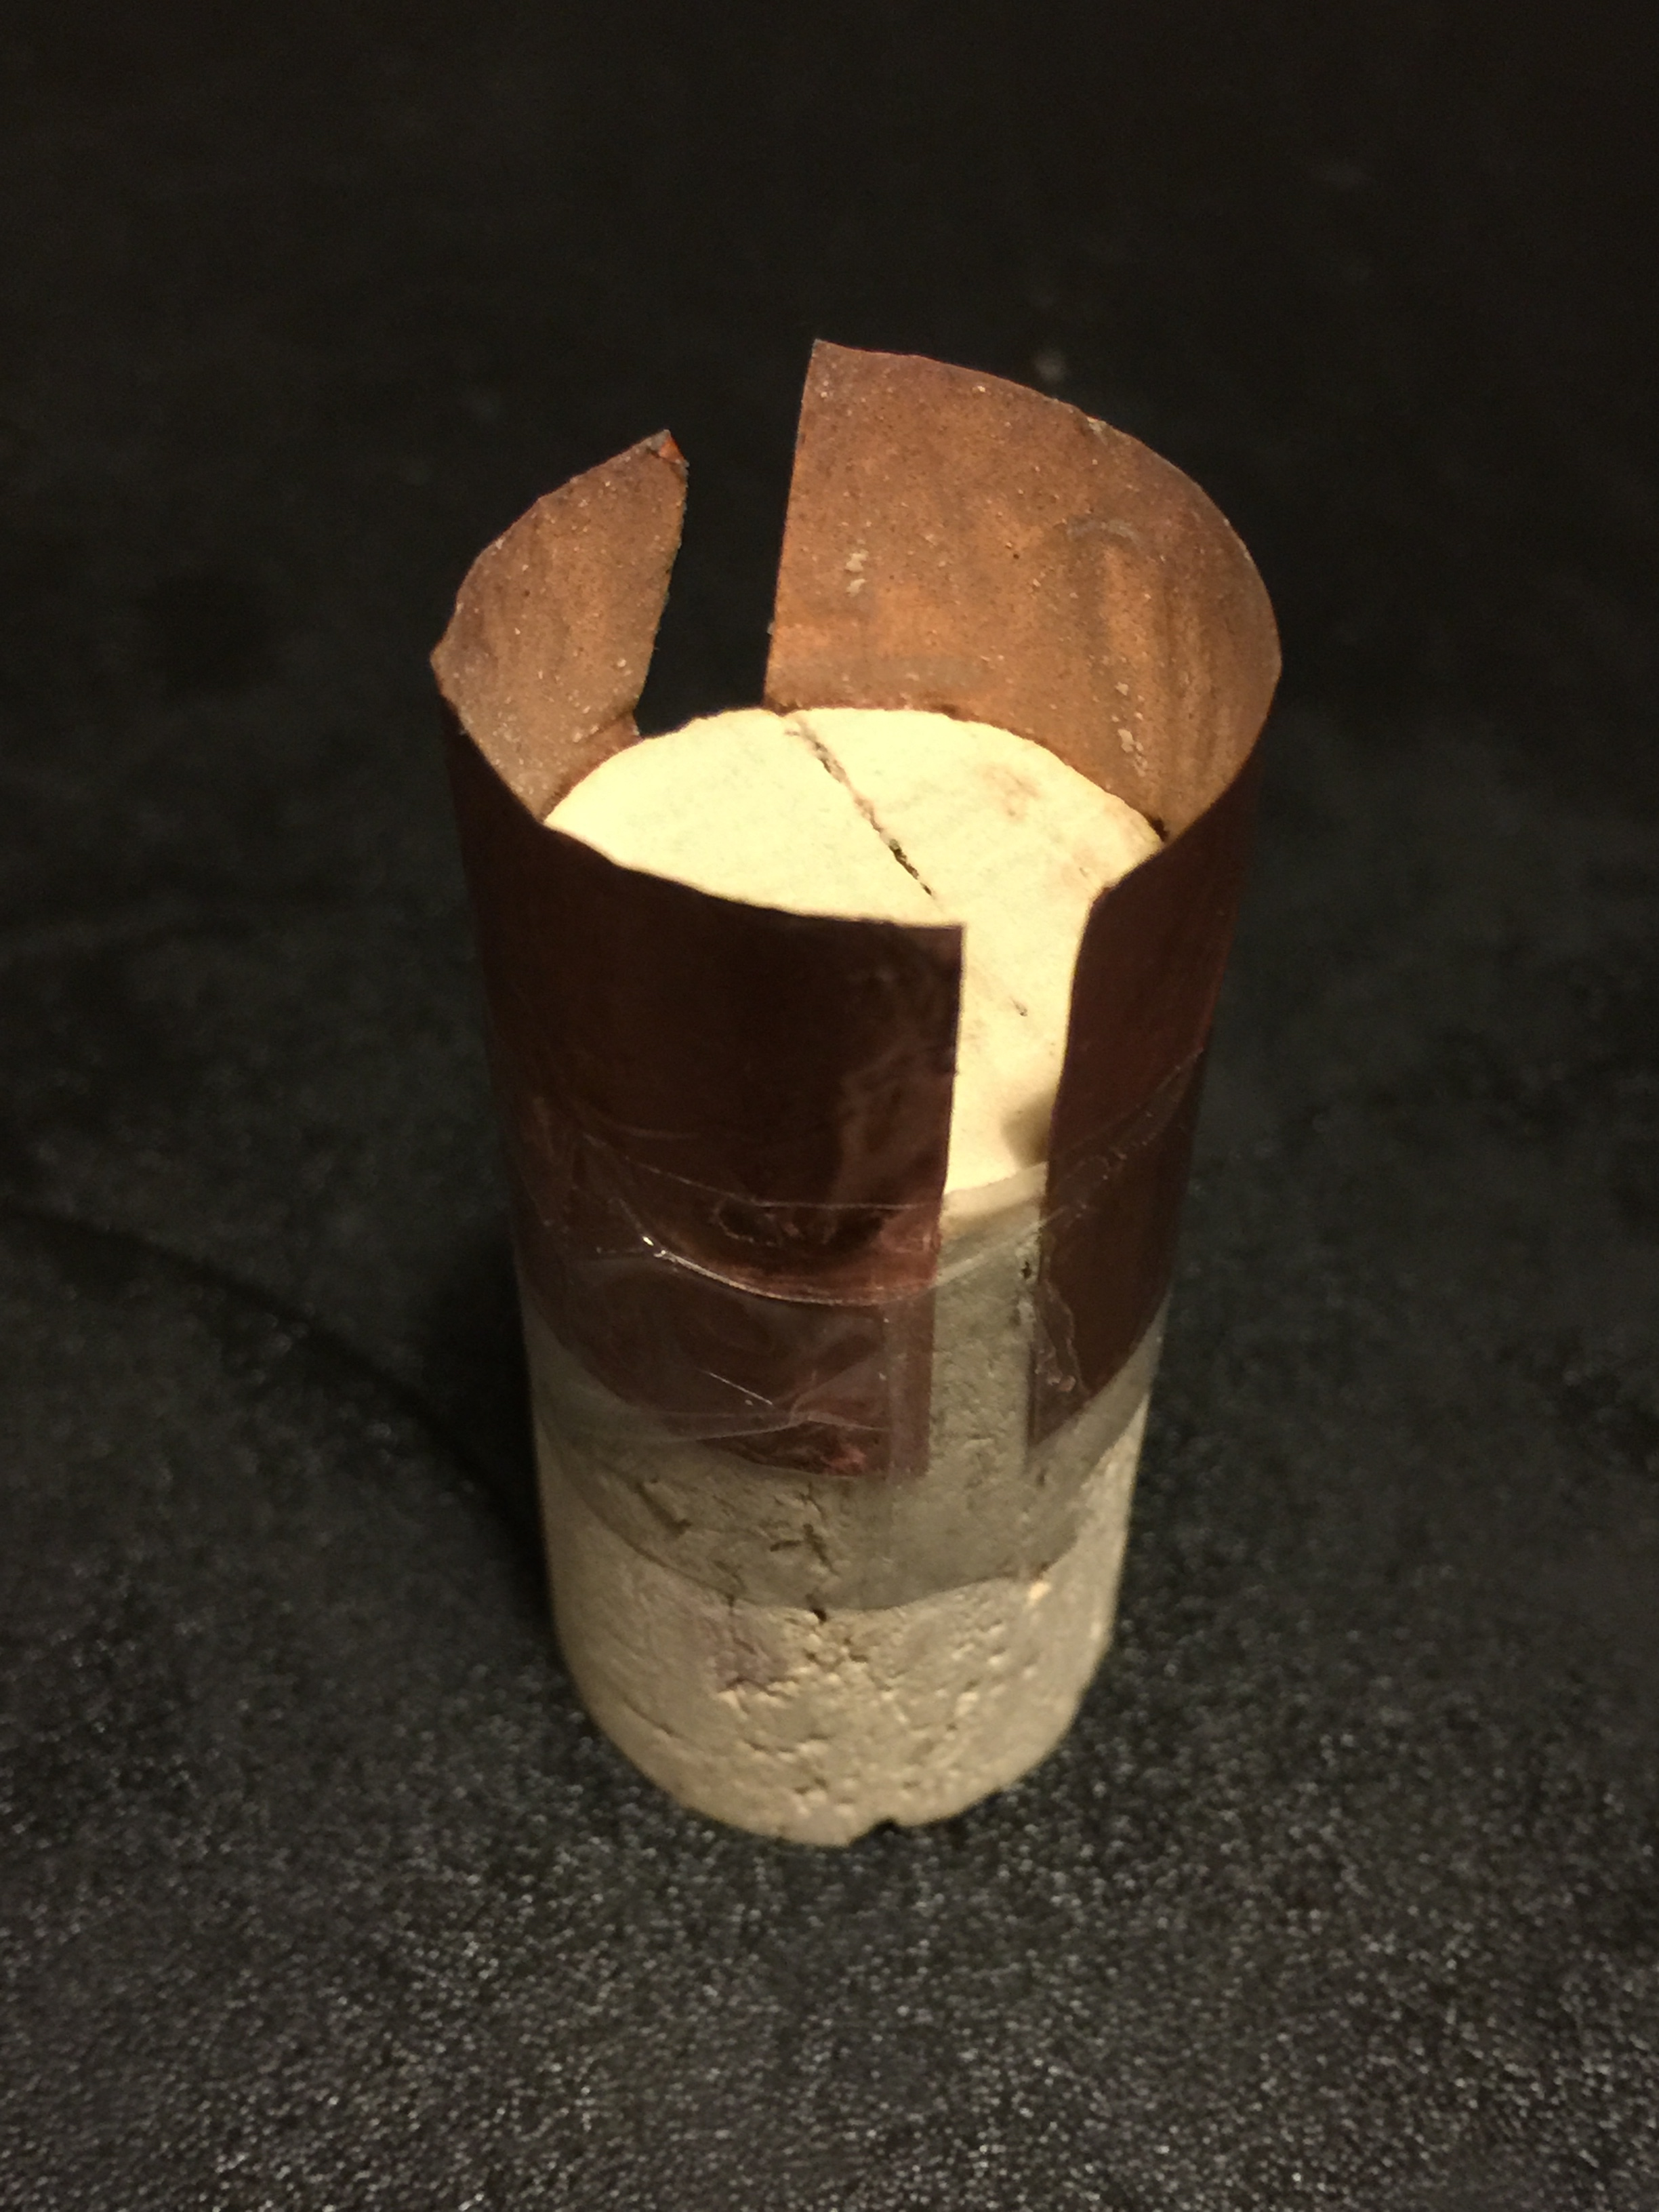
\includegraphics[width=0.5\linewidth]{dc-motor-000}
    \caption{Commutator constructed from cork and 2 pieces of copper tape}
    \label{fig1}
\end{figure}


\begin{itemize}
\item You have been supplied with a cork and adhesive copper tape.
\item Attach the tape so it can be used to form a commentator
\item You may need sell tape to increase the strength of the design
\end{itemize}

\step{Add support shaft}

\begin{figure}
    \centering
    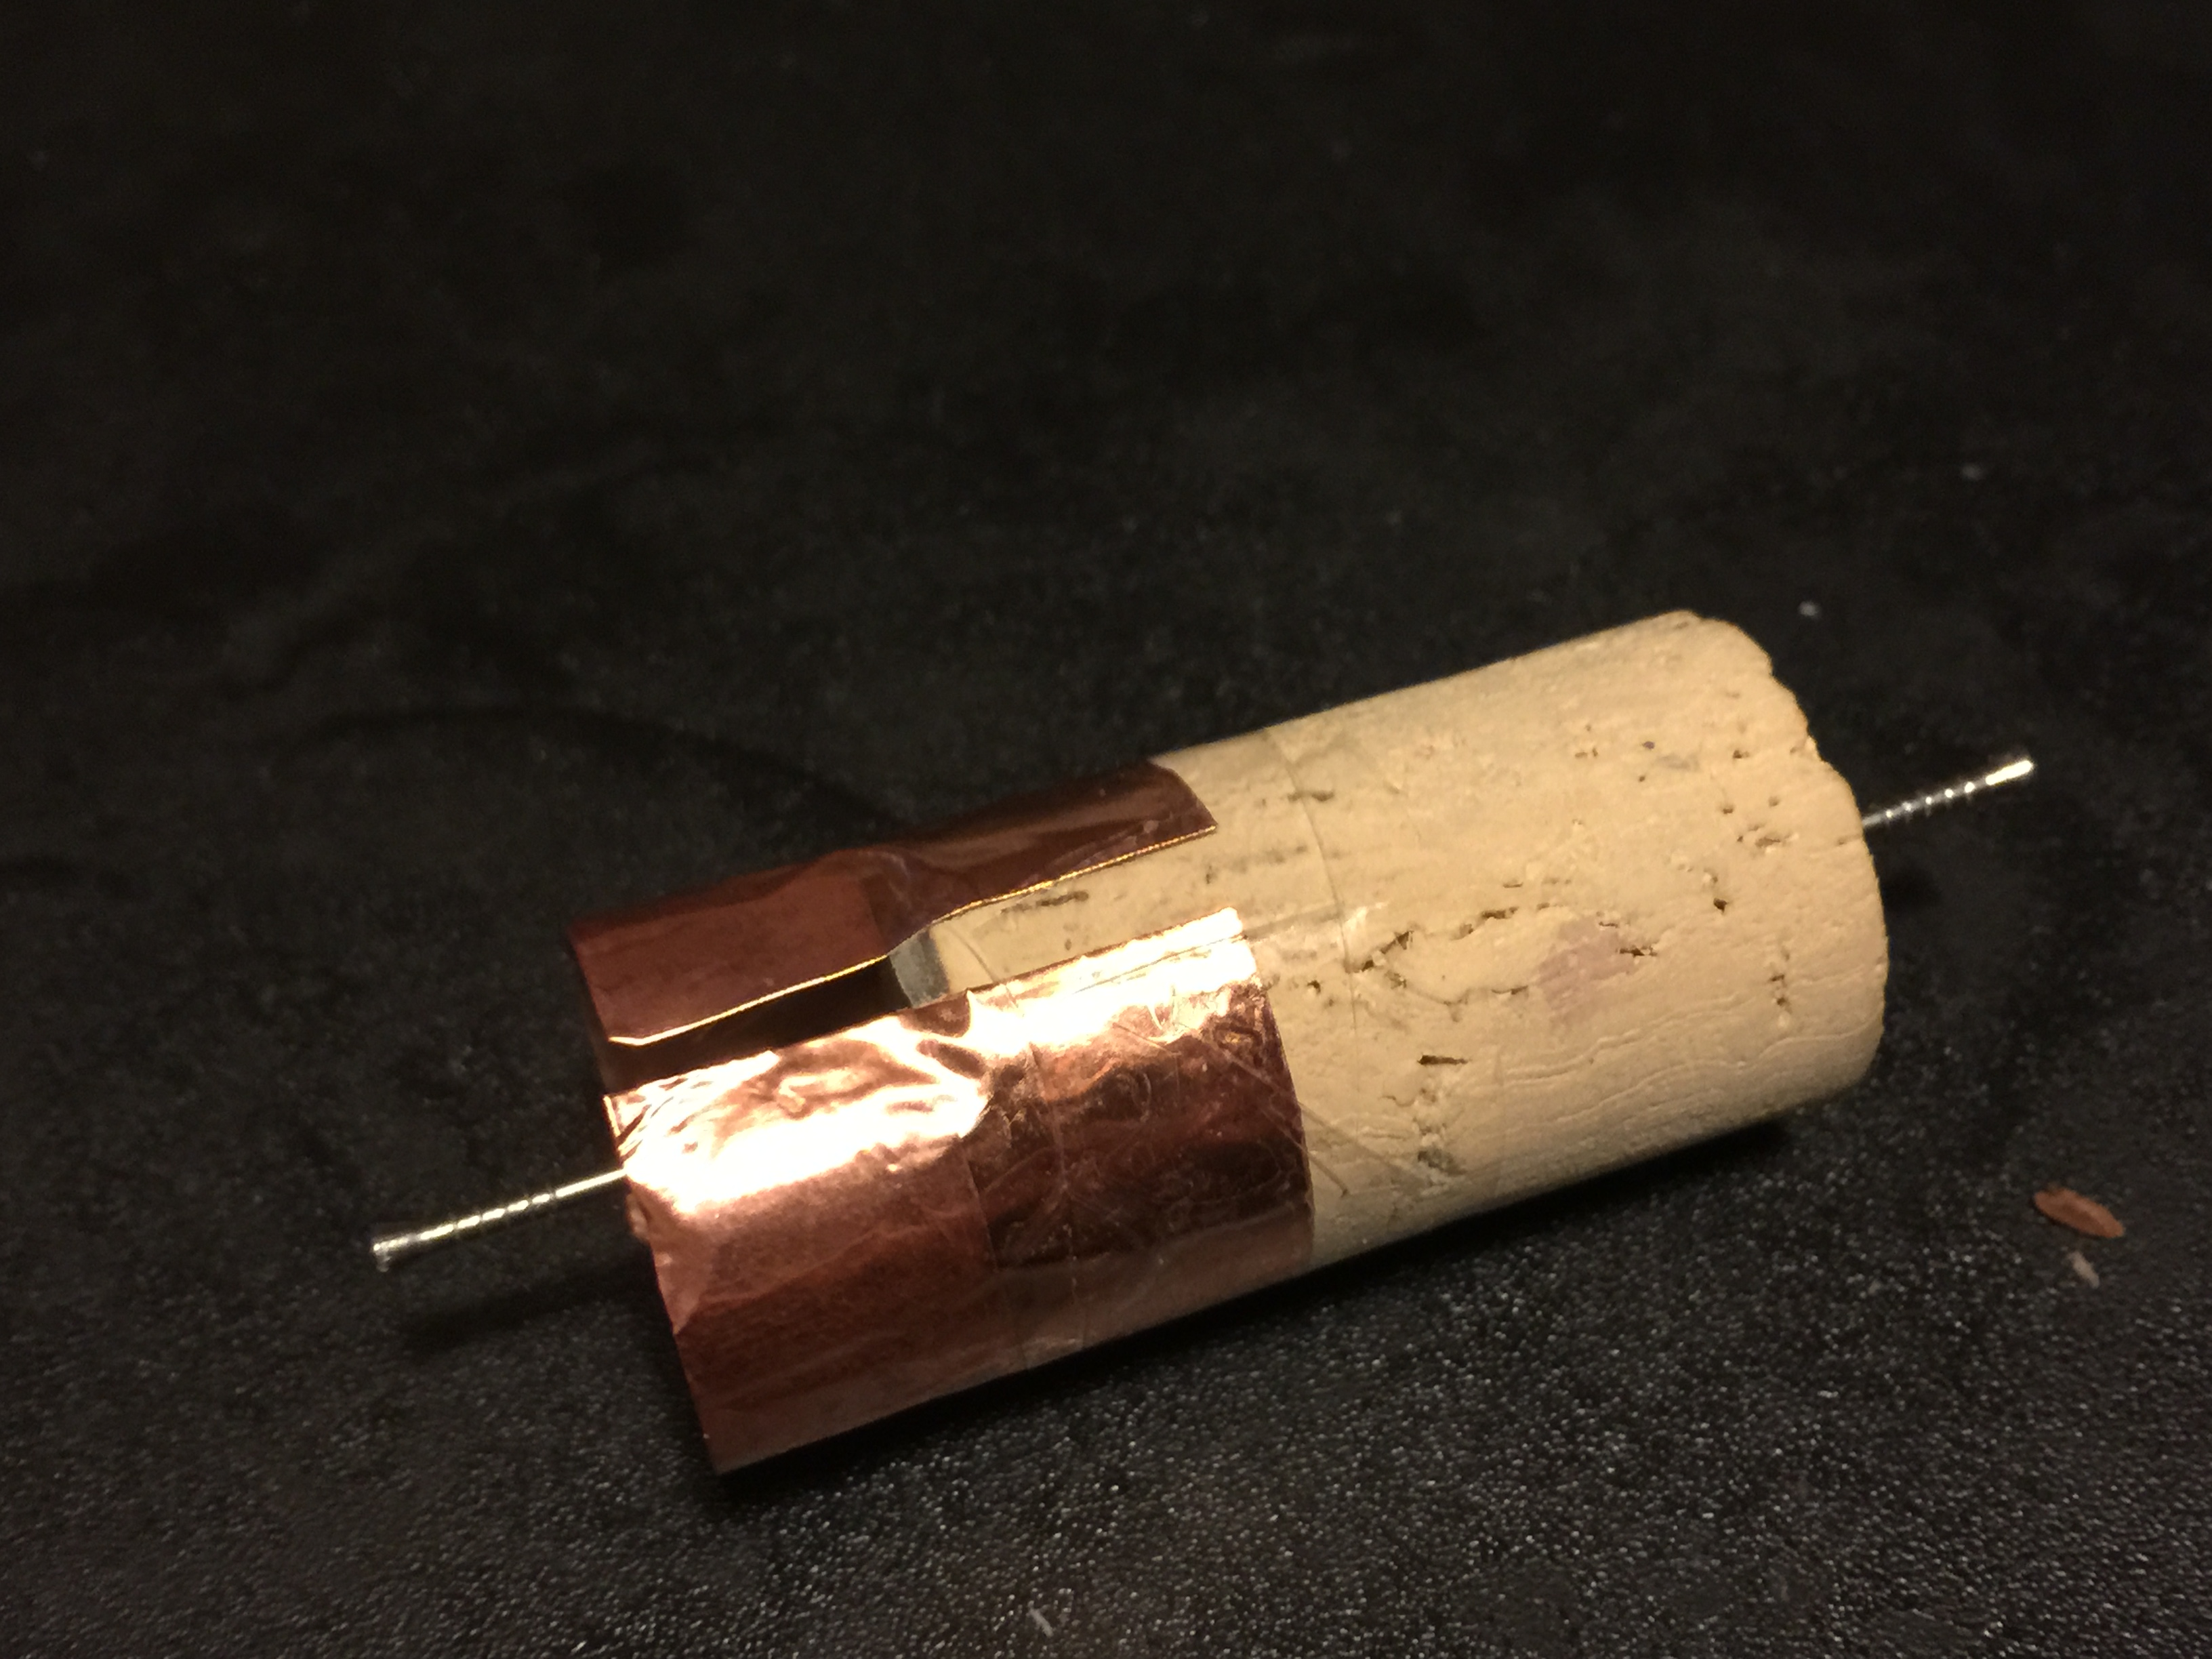
\includegraphics[width=0.8\linewidth]{dc-motor-001}
    \caption{Adding pins in armature to provide a shaft for rotation}
    \label{fig2}
\end{figure}


\begin{itemize}
\item You have been supplied with two pins.
\item Press then into opposite sides of the cork to provide a main shaft for
  the armature
\item Be careful not to damage the commutator!
\end{itemize}

\step{Wind the armature coil}

\begin{figure}
    \centering
    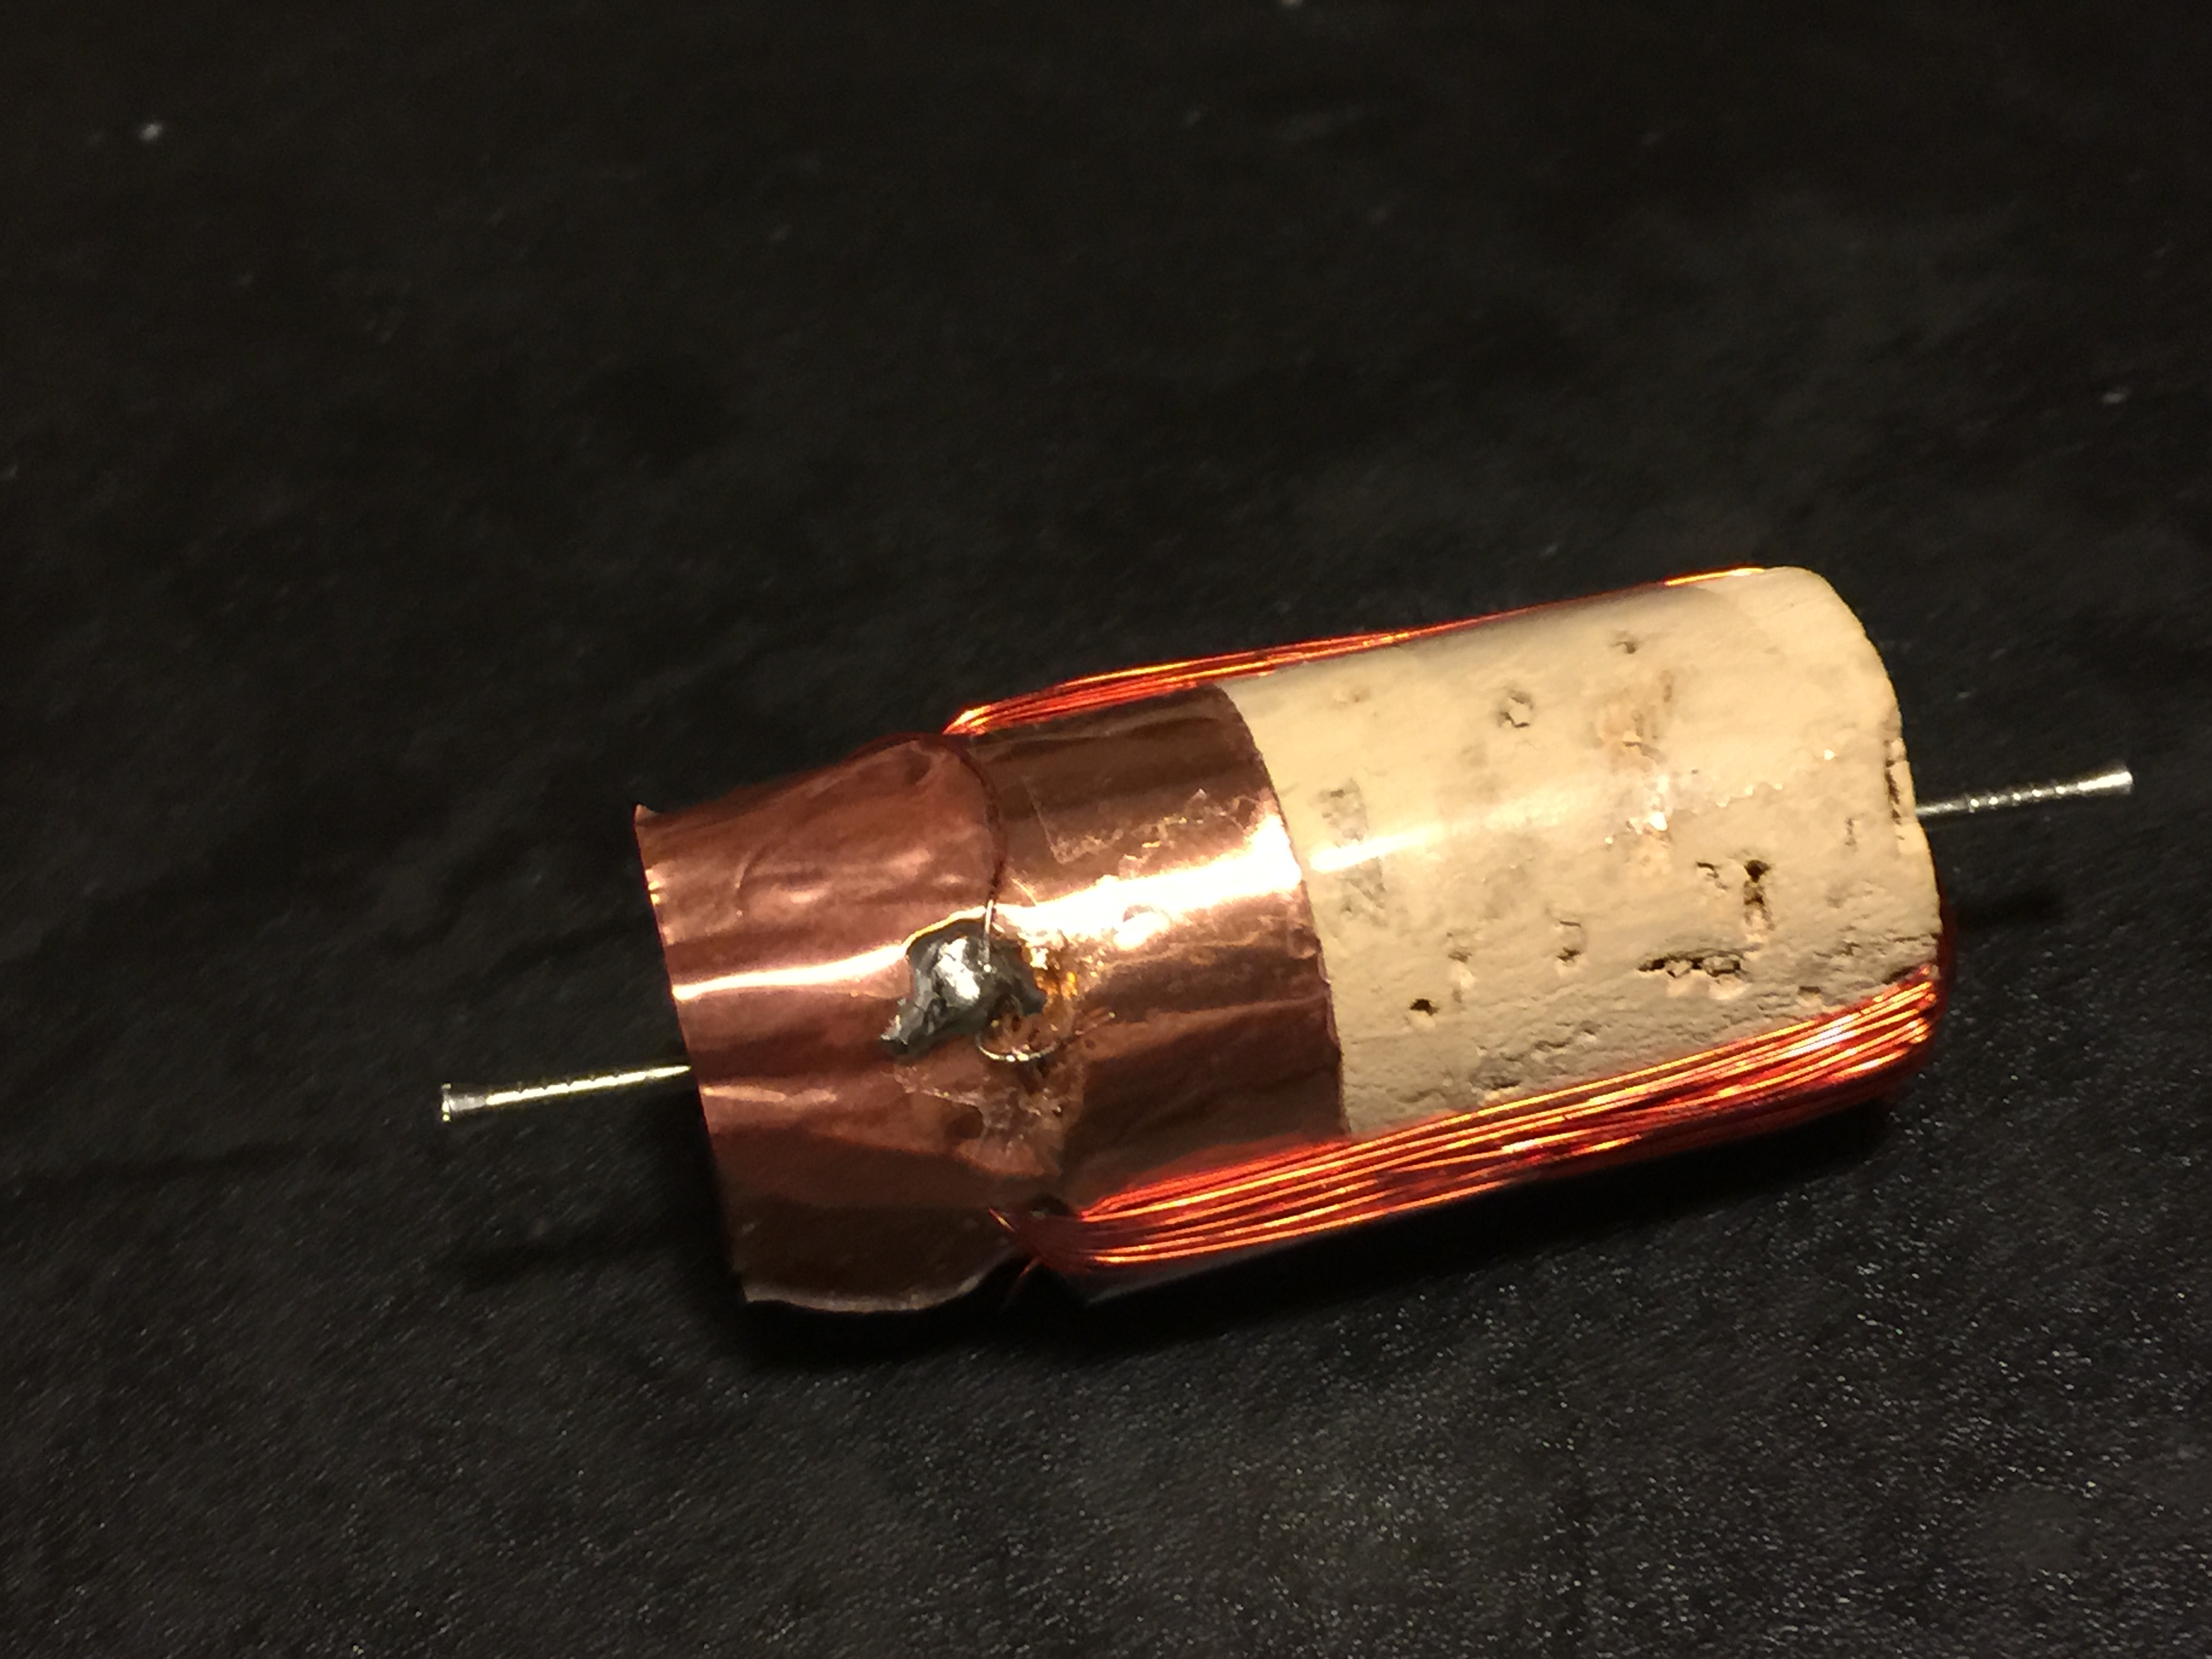
\includegraphics[width=0.6\linewidth]{dc-motor-002}
    \caption{Wind about 10m of thin copper wire around the cork to provide
    motor coil. Solder the ends to the copper commutator.}

    \label{fig3}
\end{figure}


\begin{itemize}
\item You have been supplied with about 10m of enamelled copper wire
\item Wind the wire around the cork.
\item Use sellotape to fix it down. Record how many turns you use. It should
  be at least 60 turns and preferably more.
\item Make sure both ends of the wire will remain accessible.
\item Use sandpaper to remove the enamel at the ends
\item Solder the end of the coil wires onto the copper commutator sections
\item Measure the resistance of the coil.

  \end{itemize}

\step{Build the shaft support and magnet brackets}
\begin{itemize}
\item You have been supplied with 4 large paperclips
\item Bend 2 of them so they will support the armature and allow it to
  rotate
\item Bend another 2 so they will support the neodymium magnets
\end{itemize}


\begin{figure}[!]
    \centering
    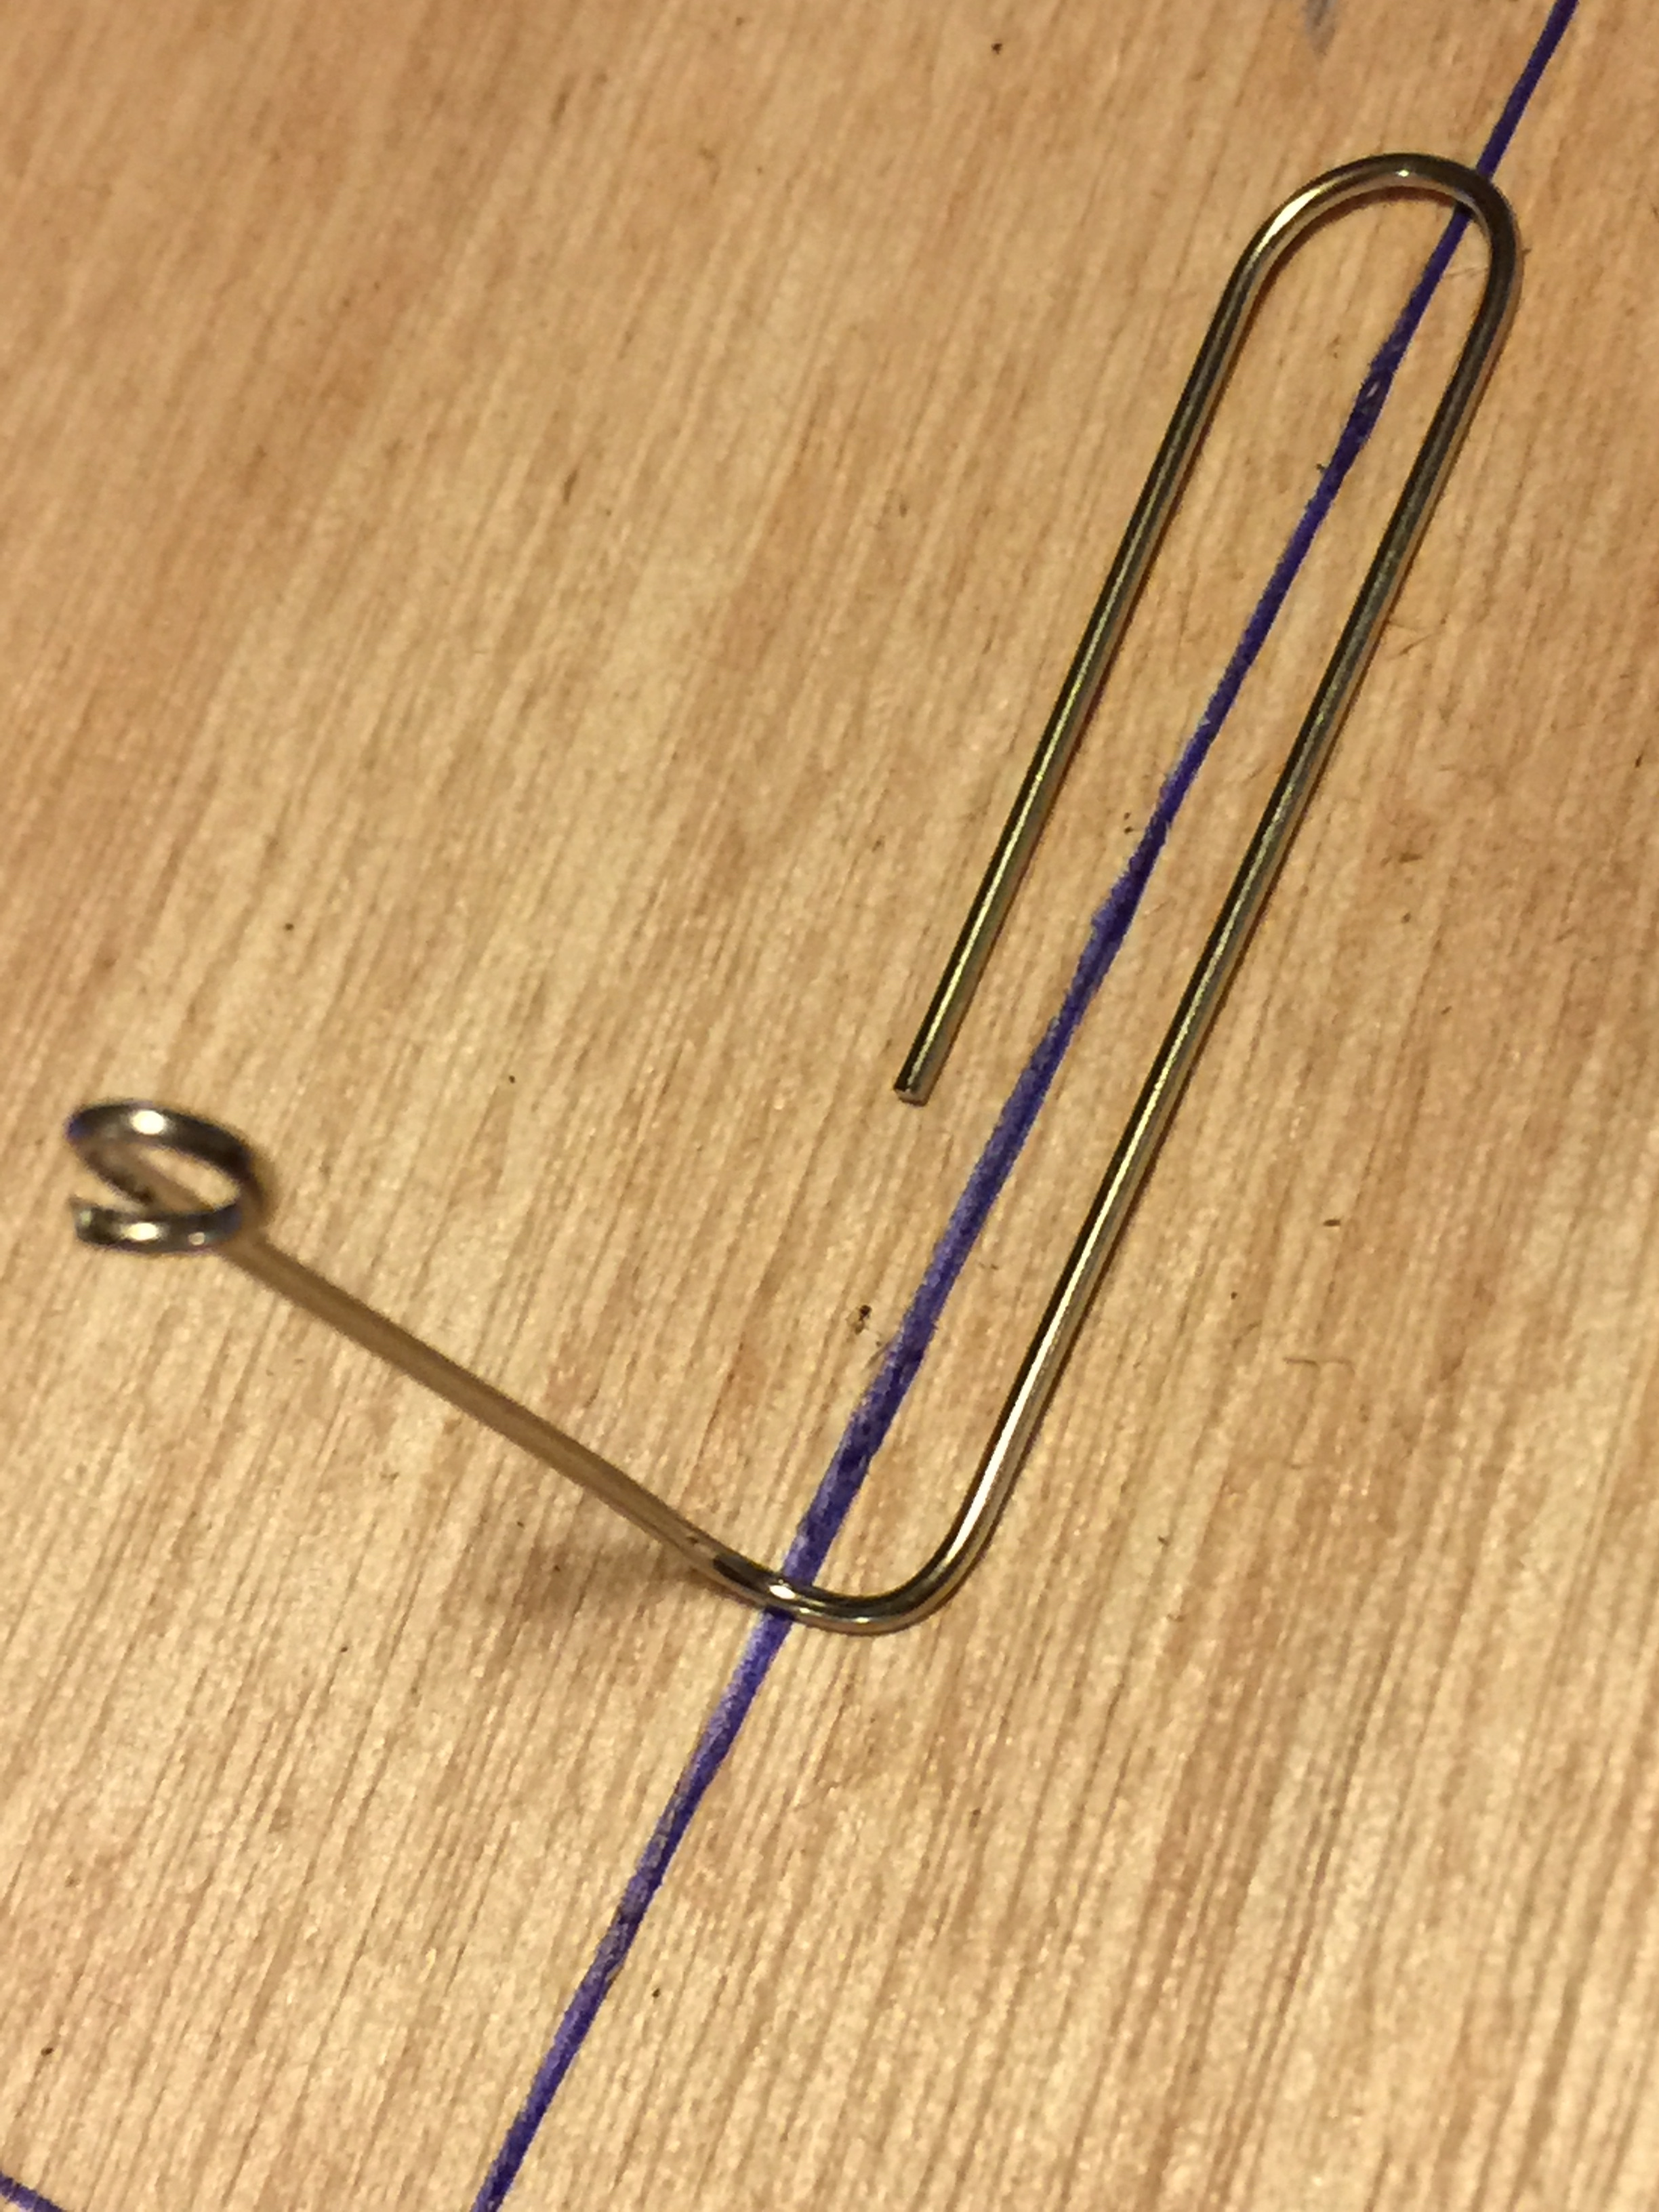
\includegraphics[width=0.4\linewidth]{dc-motor-003}
    \caption{Bend a paperclip to make 2 support bearings for the
    armature.}

    \label{fig4}
\end{figure}



\step{Build the baseplate}

\begin{figure}
    \centering
    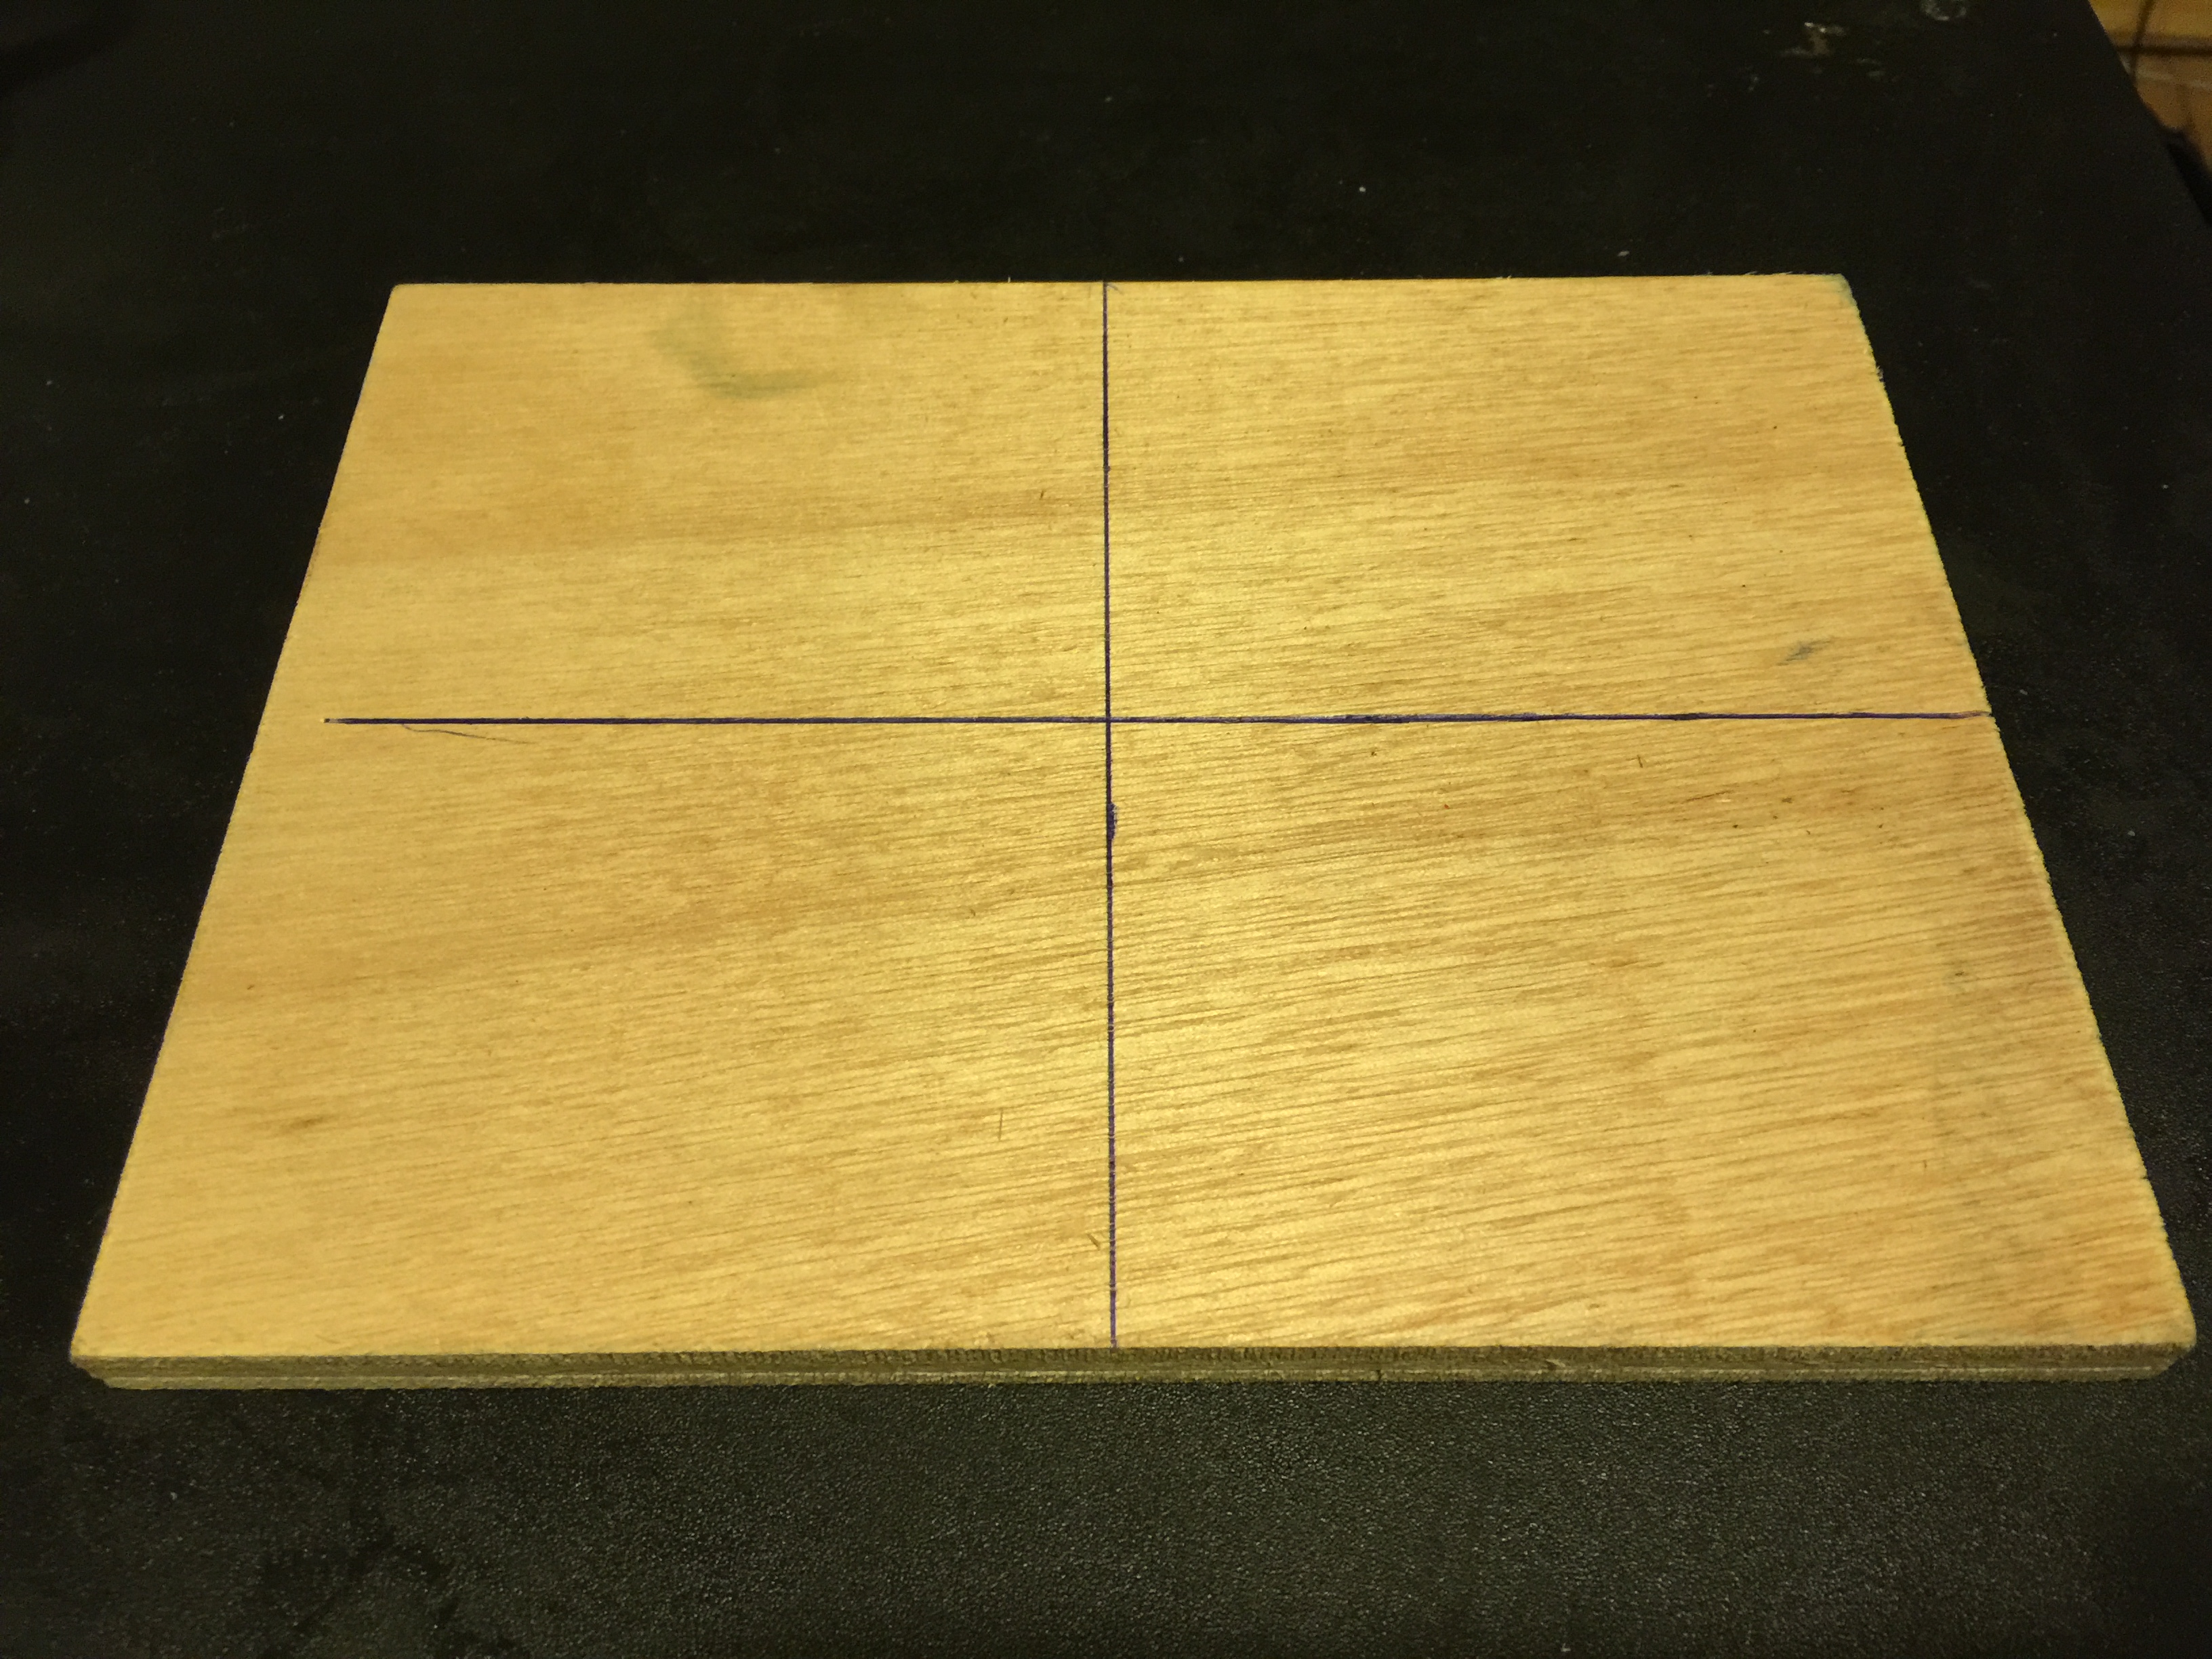
\includegraphics[width=0.8\linewidth]{dc-motor-004}
    \caption{Mark out the baseplate with perpendicular alignment lines
through its centre point.}

    \label{fig5}
\end{figure}

\begin{itemize}
\item Mark out the baseplate;
\item Provide perpendicular alignment lines through its centre point;
\item Correctly align all these parts;
\item Attach them to baseplate using the provided screws and washers;
\item Add the magnets.
\end{itemize}

Refer to figure~\ref{fig6} for the final assembly.


\part{Test the motor}

\begin{figure}
    \centering
    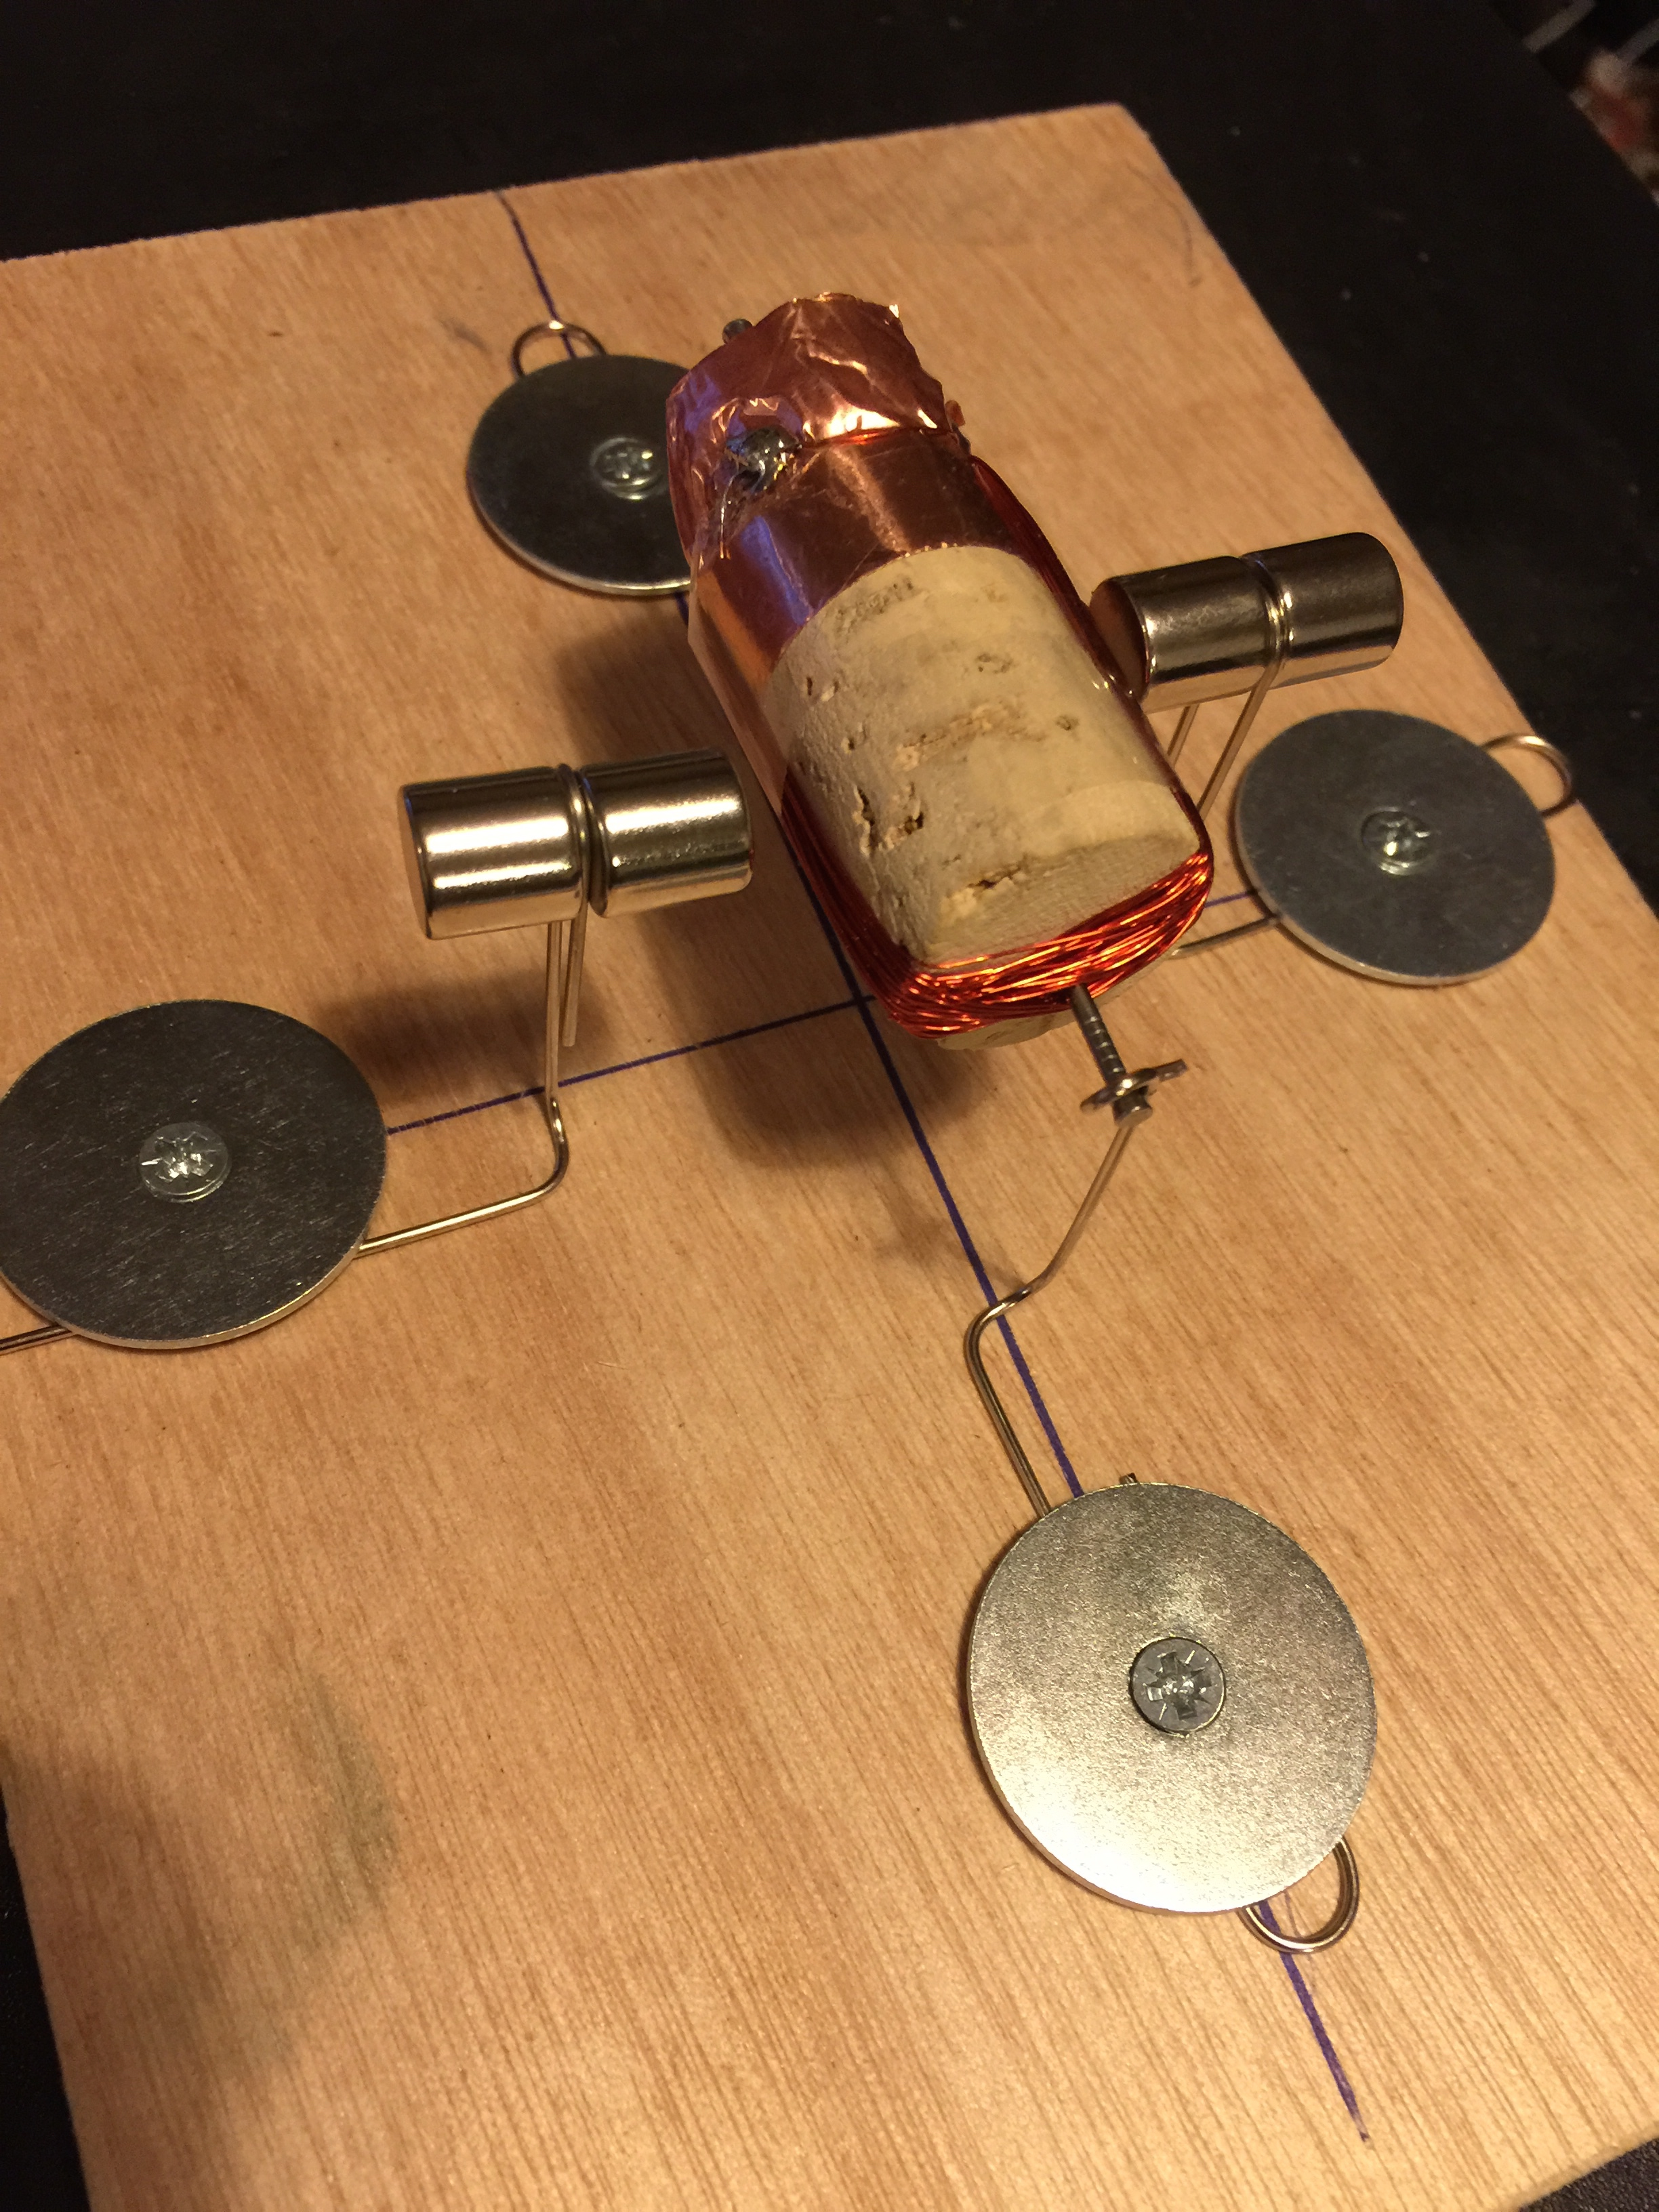
\includegraphics[width=0.5\linewidth]{dc-motor-005}
    \caption{Correctly align all that parts and screw them down to
baseplate using screws and washers provided. Add magnets and then apply
power to the commutator with stripped copper wires.}

    \label{fig6}
\end{figure}

\step{Finish the motor}

\begin{enumerate}
\item Apply power to commutator with copper wires;
\item Connect the coil to the power supply provided;
\item Notice that the power supply current is limited to 2A;
\item Be careful that the coil does not get too hot!
\item Touch wires to act like brushes on the commutation.
\end{enumerate}

\step{Test the motor}

\begin{itemize}
\item Does the armature rotate?
\item Can you measure rotational speed using modulation in armature current?
\item How fast does the motor rotate at a given applied voltage?
\end{itemize}

You might want to plot the current as a function of the voltage.

\note{

This is the right time to update your lab journal:

\begin{itemize}
    \item take pictures
    \item save your plots as image
    \item integrate them to your \texttt{journal.md} Markdown journal
    \item commit and push on GitHub
\end{itemize}
}

\part{A better DC motor}

You are now required to build a brushed DC motor \textbf{with a minimum of two
coils}. You should also build a commutator and brush mechanism so that
the motor self starts.

Further ideas to improve your design:

\begin{itemize}
\item Can you build an elegant way of holding the brushed to apply current
  to the commentator?
\item Can you improve the way the armature rotates by using better bearings?
\item How would increasing the number of turns of wire affect motor
  characteristics?
\item Consider this in terms of speed, torque and current consumption.
\end{itemize}

\textbf{You may not use parts from commercially made motors in your
designs!}

You will gain marks for improvements to the original design. For
example, by maximizing the magnetic flux passing through the armature
coils or improving the motor support and bearings.

Use your own ingenuity to come up with a design. We cannot provide
financial support for parts but you can use things you can find
yourselves. In previous years students made use of the machine shops and
3D printing facilities during this project and some of the final motors
constructed were very impressive!

You will gain marks by using a thorough test procedure and by
documenting you motor's characteristics.

\end{document}
